%% This is the ctufit-thesis example file. It is used to produce theses
%% for submission to Czech Technical University, Faculty of Information Technology.
%%
%% This is version 1.6.0, built 18. 9. 2025.
%% 
%% Get the newest version from
%% https://gitlab.fit.cvut.cz/theses-templates/FITthesis-LaTeX
%%
%%
%% Copyright 2024, Tomas Novacek
%% Copyright 2021, Eliska Sestakova and Ondrej Guth
%%
%% This work may be distributed and/or modified under the
%% conditions of the LaTeX Project Public License, either version 1.3
%% of this license or (at your option) any later version.
%% The latest version of this license is in
%%  https://www.latex-project.org/lppl.txt
%% and version 1.3 or later is part of all distributions of LaTeX
%% version 2005/12/01 or later.
%%
%% This work has the LPPL maintenance status `maintained'.
%%
%% The current maintainer of this work is Tomas Novacek (novacto3@fit.cvut.cz).
%% Alternatively, submit bug reports to the tracker at
%% https://gitlab.fit.cvut.cz/theses-templates/FITthesis-LaTeX/issues
%%
%%

% arara: xelatex
% arara: biber
% arara: xelatex
% arara: xelatex

%%%%%%%%%%%%%%%%%%%%%%%%%%%%%%%%%%%%%%%%%
% CLASS OPTIONS
% language: czech/english/slovak
% thesis type: bachelor/master/dissertation/doctoral-report
% electronic (oneside) or printed (twoside), twoside is default
% paragraph - if passed, this optional argument sets paragraphs as the deepest level of headers, styles it, numbers it and adds it to Table of Content. Use with care! Normally, it is considered unwise to use it, since it is too deep.
% colour: bw for blackwhite OR no option for default colour scheme
%%%%%%%%%%%%%%%%%%%%%%%%%%%%%%%%%%%%%%%%%
\documentclass[english,master,oneside]{ctufit-thesis}

%%%%%%%%%%%%%%%%%%%%%%%%%%%%%%%%%%
% FILL IN THIS INFORMATION
%%%%%%%%%%%%%%%%%%%%%%%%%%%%%%%%%%
\ctufittitle{Automated Security Auditing of Ethereum Smart Contracts} % replace with the title of your thesis
\ctufitauthorfull{Bc. Andrei Shchapaniak} % replace with your full name (first name(s) and then family name(s) / surname(s)) including academic degrees
\ctufitauthorsurnames{Shchapaniak} % replace with your surname(s) / family name(s)
\ctufitauthorgivennames{Andrei} % replace with your first name(s) / given name(s)
\ctufitsupervisor{Ing. Josef Gattermayer, Ph.D.} % replace with name of your supervisor/advisor (include academic degrees)
\ctufitdepartment{Katedra aplikované matematiky} % replace with the department of your defence
\ctufitprogram{Informatika} % replace with your study program
\ctufitspecialisation{Znalostní inženýrství} % replace with your specialisation
\ctufityear{2026} % replace with the year of your defence
\ctufitdeclarationplace{Prague} % replace with the place where you sign the declaration
\ctufitdeclarationdate{\today} % replace with the date of signature of the declaration
\ctufitabstractCZE{Chytré kontrakty nasazené na platformě Ethereum spravují aktiva v hodnotě miliard dolarů, což činí jejich bezpečnost kriticky důležitou. Tradiční analytické techniky pokrývají pouze část možných zranitelností a v současnosti neexistuje jediný nástroj ani metoda, která by poskytovala komplexní pokrytí všech bezpečnostních aspektů. Tato práce zkoumá, zda může retrieval-augmented generation zlepšit analýzu bezpečnosti chytrých kontraktů založenou na velkých jazykových modelech tím, že ukotví výstupy modelu v databázi známých zranitelností. Byl navržen a implementován dvoufázový systém: offline pipeline, která zpracovává zprávy o zranitelnostech, počítá jejich vektorové reprezentace a ukládá je do databáze podporující vektorové vyhledávání, a online analytická komponenta, která pro daný Solidity smart kontrakt vyhledá sémanticky podobné nálezy a použije je jako kontext pro velký jazykový model při hodnocení zranitelností. Bylo vyhodnoceno několik strategií vyhledávání napříč různými datovými sadami s cílem identifikovat nejvýkonnější konfiguraci. Výsledky ukazují, že i když se počet detekovaných zranitelností oproti základnímu modelu nezvýšil, kvalita generované analýzy se měřitelně zlepšila: věrnost se zvýšila o 37,4\% a kvalita odůvodnění o 8,3\% ve srovnání se základní variantou. Tyto poznatky naznačují, že retrieval-augmented přístup vede k lépe podloženým a přesvědčivěji odůvodněným výstupům. Závěrem jsou navrženy a diskutovány možné směry dalšího zlepšení pokrytí detekce zranitelností.}
\ctufitabstractENG{Smart contracts deployed on Ethereum manage assets worth billions of dollars, making their security critically important. Traditional analysis techniques address only a subset of possible vulnerabilities, and no single tool or method currently provides comprehensive coverage across all security aspects. This thesis investigates whether retrieval-augmented generation can enhance large language model–based smart contract security analysis by grounding model outputs in a knowledge base of known vulnerabilities. A two-stage system was designed and implemented: an offline pipeline that ingests vulnerability reports, computes vector embeddings, and stores them in a vector-enabled database, and an online analysis component that, given a Solidity smart contract, retrieves semantically similar findings and uses them as context for a large language model during vulnerability assessment. Multiple retrieval strategies were evaluated across different datasets to identify the best-performing configuration. The results show that, while the number of detected vulnerabilities did not increase compared to the baseline, the quality of the generated analysis improved measurably: faithfulness increased by 37.4\% and reasoning quality by 8.3\% relative to the baseline. These findings suggest that retrieval-augmented analysis produces more grounded and well-reasoned outputs. Future directions for improving detection coverage are also proposed and discussed.}
\ctufitkeywordsCZE{Ethereum, Solidity, Chytré Kontrakty, Detekce Zranitelností, Analýza Kódu, Velké Jazykové Modely, Generování rozšířené o vyhledávání, Vektorové Vyhledávání, Wake.}
\ctufitkeywordsENG{Ethereum, Solidity, Smart Contracts, Vulnerability Detection, Code Analysis, Large Language Models, Retrieval-Augmented Generation, Vector Search, Wake.}
%%%%%%%%%%%%%%%%%%%%%%%%%%%%%%%%%%
% END FILL IN
%%%%%%%%%%%%%%%%%%%%%%%%%%%%%%%%%%

%%%%%%%%%%%%%%%%%%%%%%%%%%%%%%%%%%
% CUSTOMIZATION of this template
% Skip this part or alter it if you know what you are doing.
%%%%%%%%%%%%%%%%%%%%%%%%%%%%%%%%%%

\RequirePackage{iftex}[2020/03/06]
\iftutex % XeLaTeX and LuaLaTeX
    \RequirePackage{ellipsis}[2020/05/22] %ellipsis workaround for XeLaTeX
\else
    \errmessage{Only compilation with XeLaTeX or LuaLaTeX is allowed}
    \stop
\fi

% hyperlinks
\hypersetup{
    pdfpagelayout=TwoPageRight,
    colorlinks=false,
    allcolors=decoration,
    pdfborder={0 0 0.1}
}

% uncomment the following to hide all hyperlinks
%\hypersetup{hidelinks}

% uncomment the following to change the colour of all hyperlinks to CTU blue
%\hypersetup{allbordercolors=decoration}

\RequirePackage{pdfpages}[2020/01/28]

%%%%%%%%%%%%%%%%%%%%%%%%%%%%%%%%%%
% CUSTOMIZATION of this template END
%%%%%%%%%%%%%%%%%%%%%%%%%%%%%%%%%%


%%%%%%%%%%%%%%%%%%%%%%
% PACKAGES SETTINGS
% You may choose to modify this part.
%%%%%%%%%%%%%%%%%%%%%%
\usepackage{dirtree}
\usepackage{graphicx}
\usepackage{lipsum,tikz}
\usepackage[style=iso-numeric]{biblatex}
\addbibresource{text/bib-database.bib}
\usepackage{xurl}
\usepackage{listings} % typesetting of sources
\usepackage{caption}
\usepackage{minted}
\usepackage{booktabs}
\usepackage{tcolorbox}
\usepackage{svg}

%%%%%%%%%%%%%%%%%%%%%%
% PACKAGES SETTINGS END
%%%%%%%%%%%%%%%%%%%%%%
\usepackage{csquotes}
\begin{document}
\frontmatter\frontmatterinit % do not remove these two commands

\thispagestyle{empty}\maketitle\thispagestyle{empty}\cleardoublepage % do not remove these four commands

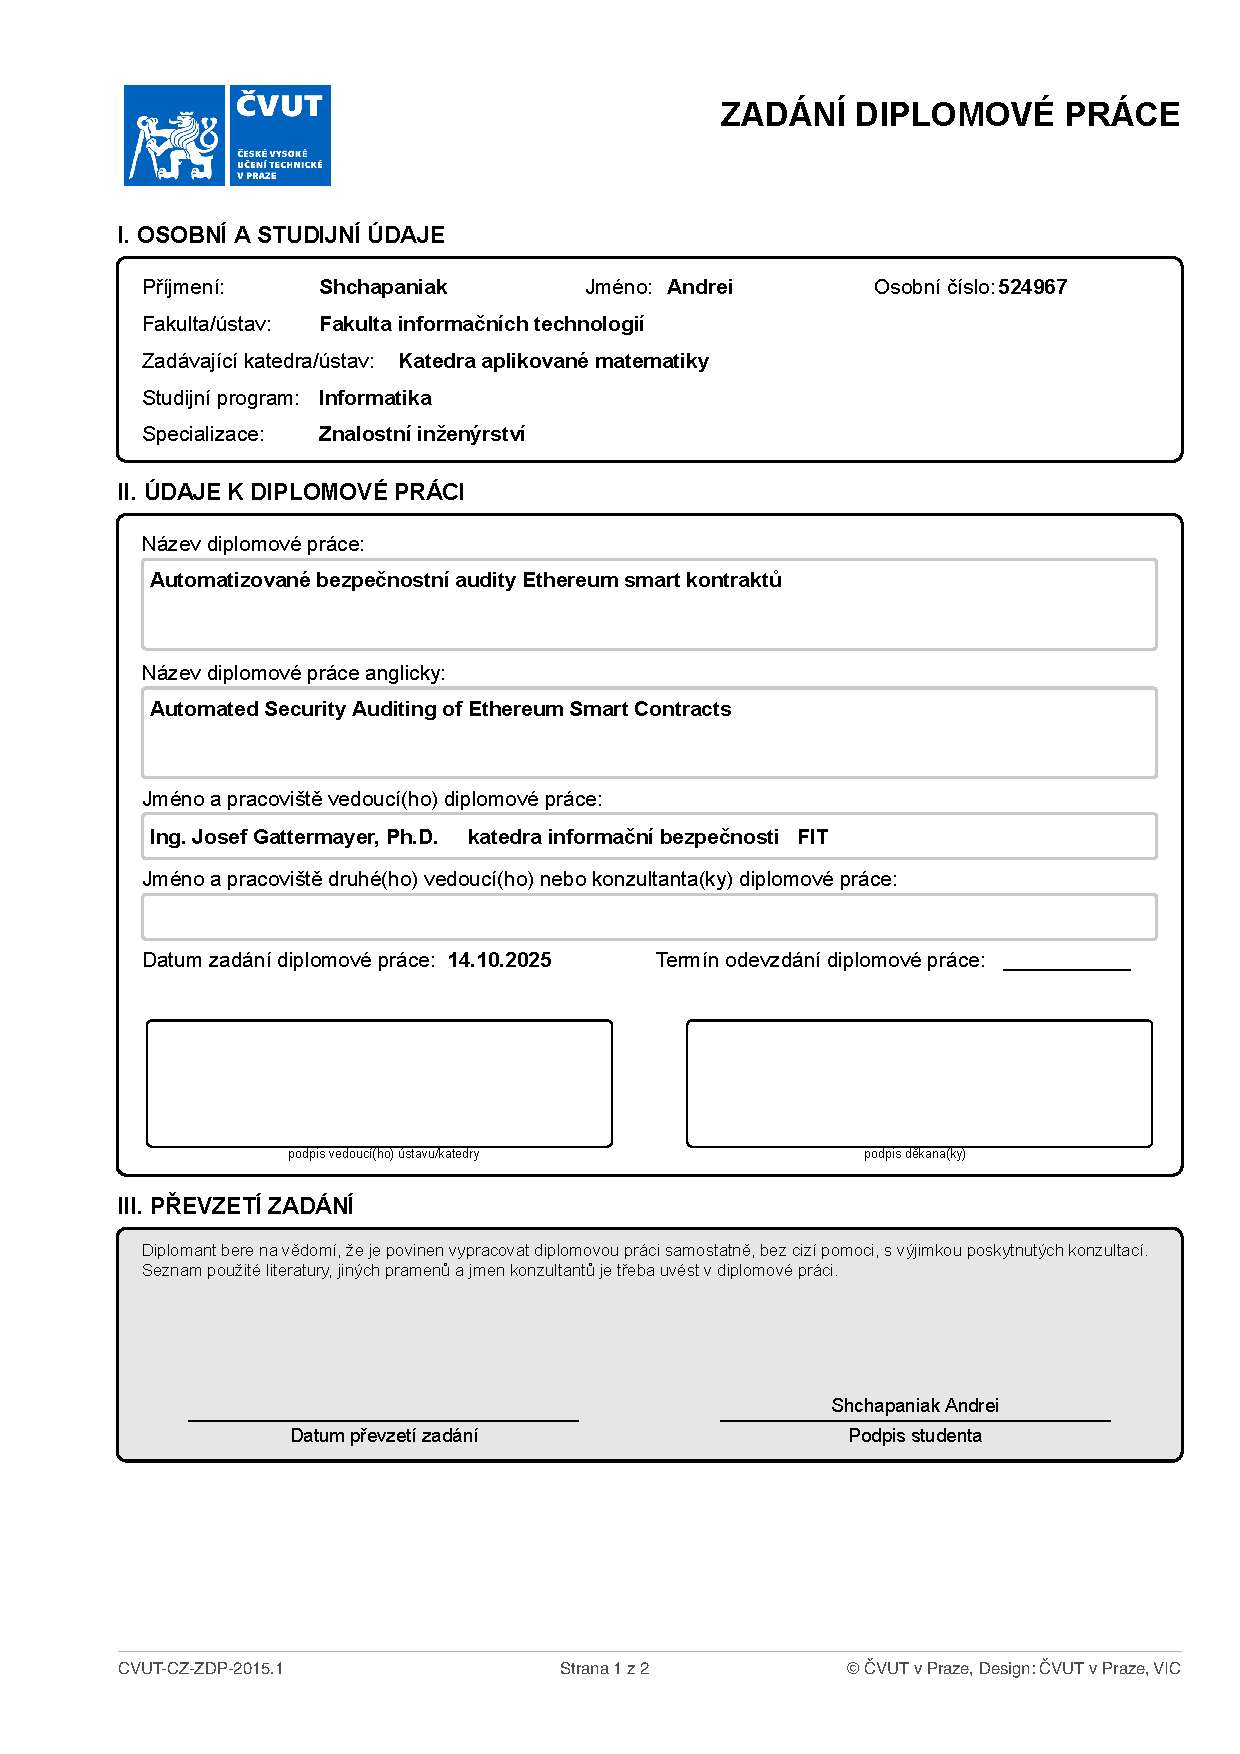
\includepdf[pages={1-}]{images/Thesis_Assignment_Andrei_Shchapaniak_Automated_Security_Auditing_of_Ethereum_Smart_Contracts.pdf} % replace this file with your thesis assignment generated from ProjectsFIT

\imprintpage % do not remove this command
\stopTOCentries

%%%%%%%%%%%%%%%%%%%
% ACKNOWLEDGMENT
% FILL IN / MODIFY
% This is a place to thank people for helping you. It is common to thank your supervisor.
%%%%%%%%%%%%%%%%%%%
\begin{acknowledgmentpage}
I would like to express my sincere gratitude to my supervisor, Ing. Josef Gattermayer, Ph.D., for providing me with the opportunity to conduct this research and for his continuous support throughout the development of this thesis. I am also deeply thankful to my family and friends, whose support helped me to be consistent through this challenging journey.
\end{acknowledgmentpage}
%%%%%%%%%%%%%%%%%%%
% ACKNOWLEDGMENT END
%%%%%%%%%%%%%%%%%%%


%%%%%%%%%%%%%%%%%%%
% DECLARATION
% FILL IN / MODIFY
%%%%%%%%%%%%%%%%%%%
% INSTRUCTIONS
% ENG: choose one of approved texts of the declaration. DO NOT CREATE YOUR OWN. Find the approved texts at https://courses.fit.cvut.cz/SFE/download/index.html#_documents (document Declaration for FT in English)
% CZE/SLO: Vyberte jedno z fakultou schvalenych prohlaseni. NEVKLADEJTE VLASTNI TEXT. Schvalena prohlaseni najdete zde: https://courses.fit.cvut.cz/SZZ/dokumenty/index.html#_dokumenty (prohlášení do ZP)
\begin{declarationpage}
I hereby declare that the presented thesis is my own work and that I have
cited all sources of information in accordance with the Guideline for adhering
to ethical principles when elaborating an academic final thesis. I declare that
I have used AI tools during the preparation and writing of my thesis. I have
verified the generated content. I confirm that I am aware that I am fully
responsible for the content of the thesis. I acknowledge that my thesis is
subject to the rights and obligations stipulated by the Act No. 121/2000
Coll., the Copyright Act, as amended, in particular the fact that the Czech
Technical University in Prague has the right to conclude a license agreement
on the utilization of this thesis as a school work pursuant of Section 60 (1) of the Act.
\end{declarationpage}
%%%%%%%%%%%%%%%%%%%
% DECLARATION END
%%%%%%%%%%%%%%%%%%%

% Use one of the two following commands. The first prints abstracts+keywords on two pages, the second puts them on one page (if possible). \printonepageabstract can also accept optional argument that specifies a vertical space before both abstracts (the default is 18 mm).
\printtwopageabstract
%\printonepageabstract 

%%%%%%%%%%%%%%%%%%%
% SUMMARY
% FILL IN / MODIFY
% OR REMOVE ENTIRELY (upon agreement with your supervisor)
% (appropriate to remove in most theses)
%%%%%%%%%%%%%%%%%%%
% \begin{summarypage}
% \section*{Summary section}
% 
% \lipsum[1][1-8]
% 
% \section*{Summary section}
% 
% \lipsum[2][1-6]
% 
% \section*{Summary section}
% 
% \lipsum[3]
% 
% \section*{Summary section}
% 
% \lipsum[2]
% 
% \section*{Summary section}
% 
% \lipsum[1][1-8] Lorem lorem lorem.
% \end{summarypage}
%%%%%%%%%%%%%%%%%%%
% SUMMARY END
%%%%%%%%%%%%%%%%%%%

\tableofcontents % do not remove this command
%%%%%%%%%%%%%%%%%%%%%%
% list of other contents: figures, tables, code listings, algorithms, etc.
% add/remove commands accordingly
%%%%%%%%%%%%%%%%%%%%%%
\listoffigures % list of figures
\begingroup
\let\clearpage\relax
\listoftables % list of tables. Remove if you do not have any.
\thectufitlistingscommand{} % list of code listings. Remove if you do not have any.
\thectufitlistofalgorithmscommand{} % list of algorithm pseudocodes defined using the algorithm package.
\endgroup
%%%%%%%%%%%%%%%%%%%%%%
% list of other contents END
%%%%%%%%%%%%%%%%%%%%%%

%%%%%%%%%%%%%%%%%%%
% ABBREVIATIONS
% FILL IN / MODIFY
% OR REMOVE ENTIRELY
% List the abbreviations in lexicography order.
%%%%%%%%%%%%%%%%%%%
\chapter{\thectufitabbreviationlabel}

\begin{tabular}{rl}
    AI & Artificial Intelligence\\
    dApps & decentralized applications\\
    EOA & Externally Owned Account\\
    EVM   & Ethereum Virtual Machine\\
    LLM   & Large Language Model\\
    PoW & Proof of Work\\
    PoS & Proof of Stake\\
\end{tabular}
%%%%%%%%%%%%%%%%%%%
% ABBREVIATIONS END
%%%%%%%%%%%%%%%%%%%
\resumeTOCentries
\mainmatter\mainmatterinit % do not remove these two commands
%%%%%%%%%%%%%%%%%%%
% THE THESIS
% MODIFY ANYTHING BELOW THIS LINE
%%%%%%%%%%%%%%%%%%%

\include{text/text} % include `text.tex' from `text/' subdirectory

\appendix\appendixinit % do not remove these two commands

\include{text/appendix} % include `appendix.tex' from `text/' subdirectory

\backmatter % do not remove this command

\begingroup
\raggedright
\printbibliography % print out the BibLaTeX-generated bibliography list
\endgroup

\chapter{Contents of the attachment}

    \dirtree{%
        .1 /.
        .2 README.md\DTcomment{brief description of the medium contents}.
        .2 src\DTcomment{source code of the implementation}.
        .3 alembic/\DTcomment{database migration scripts}.
        .3 data/\DTcomment{evaluation datasets and golden findings}.
        .3 sql/\DTcomment{auxiliary SQL queries}.
        .3 tests/\DTcomment{automated tests (pytest)}.
        .3 rag\_eval/.
        .4 cli.py\DTcomment{Click CLI entry point}.
        .4 config.py\DTcomment{settings, embedding profiles, labels}.
        .4 datasets/\DTcomment{data ingestion, embedding, preprocessing}.
        .4 db/\DTcomment{SQLAlchemy models and repository layer}.
        .4 experiments/\DTcomment{experiment tracking}.
        .4 generation/\DTcomment{LLM-as-judge classification and evaluation}.
        .4 llm/\DTcomment{LLM provider abstraction}.
        .4 pipeline/\DTcomment{end-to-end evaluation pipeline runner}.
        .4 retrieval/\DTcomment{search service, vector store, reranking}.
        .3 pyproject.toml\DTcomment{project metadata and dependencies}.
        .3 alembic.ini\DTcomment{Alembic configuration}.
        .3 Makefile\DTcomment{common development commands}.
        .3 .env.example\DTcomment{environment variable template}.
        .2 thesis.
        .3 src/\DTcomment{\LaTeX{} source files of the thesis}.
        .3 thesis.pdf\DTcomment{compiled thesis in PDF format}.
    }
 % include `medium.tex' from `text/' subdirectory

\end{document}
